\section{Contrastive Language-Image Pre-training (CLIP)}
% As our model is built based on CLIP models, we first provide a brief review of model architectures and training settings in CLIP.
We first provide a brief review of model architectures and training settings in CLIP.

CLIP uses two separate models for image encoder and text encoder respectively. For text inputs, a 12-layer Transformer is adopted with 512 width and 8 attention heads. Raw texts are first converted using byte pair encoding~\cite{bpe} technique under a vocabulary size of 49,152. The text sequence length is capped at 76 and added by a positional encoding before being sent into the text encoder. On the other hand, CLIP has different versions of image encoder with ResNet-based and Vision Transformer-based architectures. As the following researches have demonstrated the better performances of Vision Transformer models, we only consider Transformer-based image encoders in this paper. Similar to the text input, images are first converted to patches, and added by a positional encoding. At the last stage of both encoders, a global pooling function is adopted to compress the feature map into a single feature, which serves as the representation of the whole image/text sequence. The cosine distance of the image and text features is computed as the similarity of the data pair. For training supervision, a contrastive loss is adopted to maximize the similarity of matched pairs while minimizing the similarity of unmatched pairs. Given a batch of $N$ data pairs $\{{\rm I}_i, {\rm T}_i\}_{i=1}^N$, where $I_i$ and ${\rm T}$ represents the $i_{\rm th}$ image and text respectively, the loss function can be parameterized as:

% \begin{equation}
%     s(I, T) = {\rm cos}(f_i(I), f_t(T)),
% \end{equation}
\begin{equation}
    L = -\frac{1}{2}\sum_{i=1}^N \left({\rm log}\frac{{\rm exp}({\rm cos}(f_{\rm I}({\rm I}_i), f_{\rm T}({\rm T}_i))/\tau)}{\sum_{j=1}^N{\rm exp}({\rm cos}(f_{\rm I}({\rm I}_i), f_{\rm T}({\rm T}_j))/\tau)}+{\rm log}\frac{{\rm exp}({\rm cos}(f_{\rm I}({\rm I}_i), f_{\rm T}({\rm T}_i))/\tau)}{\sum_{j=1}^N{\rm exp}({\rm cos}(f_{\rm I}({\rm I}_j), f_{\rm T}({\rm T}_i))/\tau)}\right),
\end{equation}
where $f_{\rm I}$ and $f_{\rm T}$ correspond to image and text encoders respectively, ${\rm cos}(\cdot)$ denotes the cosine similarity between the inputs, and $\tau$ is a learnable temperature initialized at $0.07$.

This simple training framework actually brings several concerns that need to be addressed. First, the pre-training framework fails to model the semantic information of inputs due to the simplicity of the data structure. This results in inferior performances on tasks that require reasoning ability, \textit{e.g.}, visual question answering and visual commonsense reasoning. Second, the image and text features reside in separate spaces, which makes it difficult to model the interactions between different modalities. Third, the massive time and resource consumption in the training procedure set restrictions on performing a full pre-training schedule from scratch.

\begin{figure}[t]
  \centering
  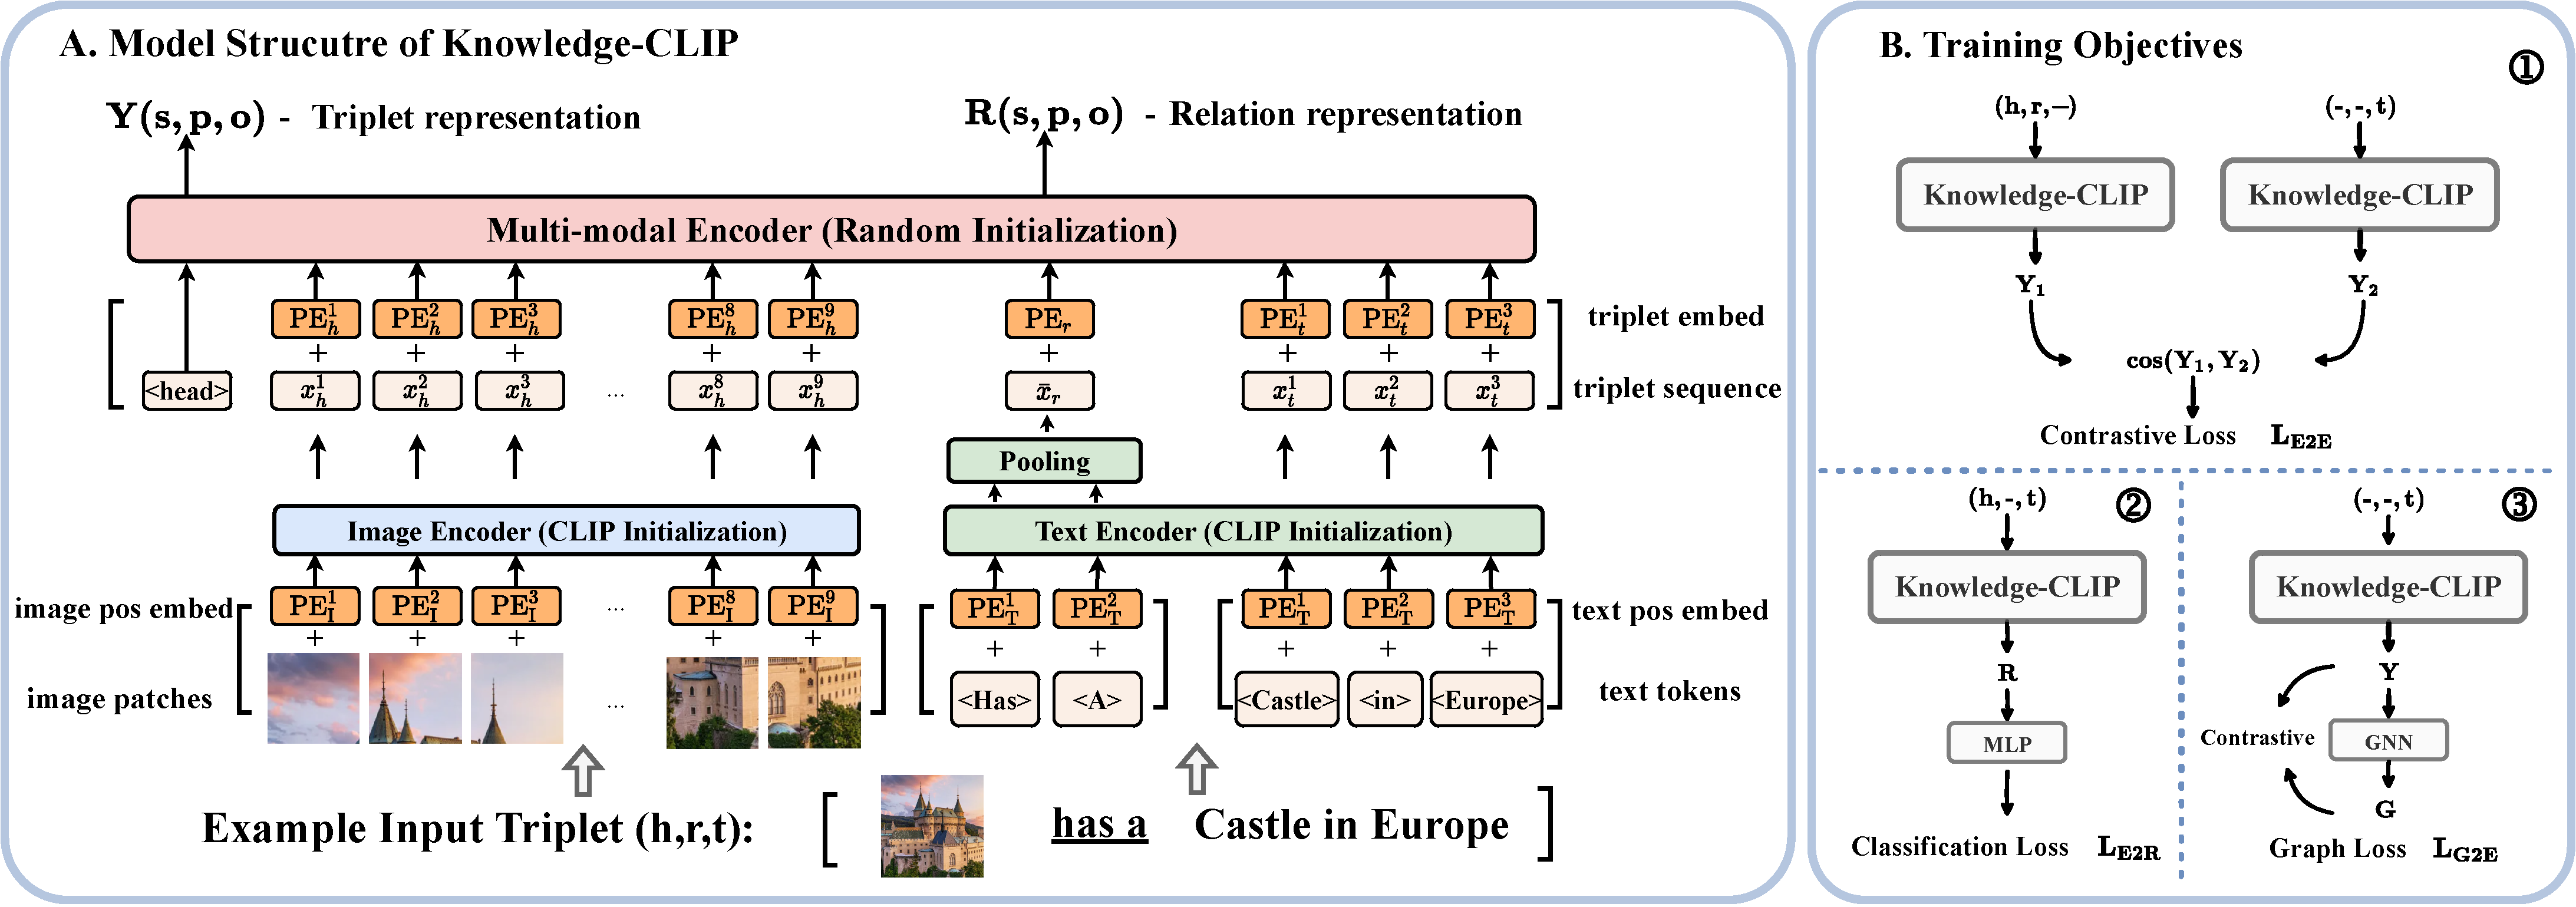
\includegraphics[width=1.0\linewidth]{3_5.pdf}
%   \vskip -0.1in
  \caption{An overview of our framework. (A) Given a data triplet $h,r,t$ with entities $h,t$ and their relation $r$, image and text encoders first extract raw features, then a multi-modal encoder consumes the concatenated triplet sequence and outputs triplet and relation representations. (B) Three types of training objectives adopted in our framework.}
%  \vskip -0.05in  
\label{fig3}
\end{figure}

\section{Knowledge-CLIP}
\label{sec:method}

% As we have summarized above, there are several concerns that hinder the transferability to several downstream tasks and potential improvements on CLIP model structures. In this paper, we address these limitations by proposing a knowledge-enhanced pre-training framework, which endows CLIP models with higher generalization power

As we have summarized above, there are several concerns that hinder the transferability of CLIP and potential improvements on model performances. In this paper, we propose a novel pre-training framework based on knowledge graphs, that addresses the limitation of the original CLIP model from several perspectives: (1) we introduce knowledge graphs into the training dataset where the graph-structured data and semantic relations between concepts enable the model to extract semantic features and establish semantic connection across inputs; (2) A multi-modal encoder is added on top of the current image and text encoders to fuse the features from different modalities, and model the joint distribution between inputs; (3) A continuous learning strategy based on the pre-trained model of CLIP is adopted which avoids the massive computation cost in the pre-training procedure, and enhance the generalization power of the model efficiently. We introduce our framework in detail in the following sections, and show the overview in Fig.~\ref{fig3}.

\subsection{Data Preparation}
Different from raw image-text pairs adopted in the original CLIP, our model takes knowledge graphs as input. A knowledge graph can be defined as a directed graph $\mathcal{G}=\{\xi, \mathcal{R}, \mathcal{T}_\mathcal{R}\}$, where $\xi$, $\mathcal{R}$ correspond to sets of entities and relations, and $\mathcal{T}_\mathcal{R}$ represent the set of relation triplets. A triplet $(h,r,t)\in \mathcal{T}_\mathcal{R}$ denotes that entity $h\in \xi$ has relation $r\in \mathcal{R}$ with entity $t \in \xi$. As illustrated in Fig.~\ref{fig2}, we pre-train our model on three types of knowledge graphs, including multi-modal knowledge graph, scene graph, and language-based knowledge graph. Among these, relations are constantly described in language tokens, where the entities are from different modalities in different forms.

For multi-modal knowledge graph, the entities contain both illustrative images and language descriptions. Through representing the same entity under various modalities and connecting entities with relations, it helps to build semantic connections between vision and language concepts. In practice, language and vision descriptions are randomly chosen for each entity. In this way, the triplet set $\mathcal{T}_\mathcal{R}$ contains different forms including (Img, Rel, Img), (Img, Rel, Text), and (Text, Rel, Text), providing rich information across modalities while also enhancing perceptions within modalities. 

Different from multi-modal knowledge graph, scene graph extracts visual concepts (mainly objects) for each image, and connects them with predefined semantic relations describing relative locations, actions, etc. Therefore, the entities in the scene graph correspond to a certain region in an image, with the triplet form of (Img, Rel, Img). We practically use the selected regions as the input and discard the irrelevant parts. As two entities in the same triplet denote different regions in the same image, it forces the model to extract more fine-grained features.

Lastly, language-based knowledge graph connects words and phrases of natural language with labeled edges. It is built on only language modality with the triplet form of (Text, Rel, Text), while helping to build semantic alignment within word tokens.

% \noindent
% \textbf{VisualSem}~\cite{visualsem} is a high-quality multi-modal knowledge graph dataset for vision and language concepts. VisualSem includes entities with multilingual glosses, multiple illustrative images, and visually relevant relations, covering a total number of 90k nodes, 1.3M glosses and 938k images. 13 semantic relations are used to connect different entities in the graph, while the entities in VisualSem are linked to Wikipedia articles, WordNet~\cite{wordnet}, and high-quality images from ImageNet~\cite{imagenet}. Through representing the same entity under various modalities and connecting entities with relations, VisualSem helps to build semantic connections between vision and language concepts. In practice, language and vision descriptions are randomly chosen for each entity, while the relations are all in language form. In this way, the triplet set $\mathcal{T}_\mathcal{R}$ contains different forms including (Img, Rel, Img), (Img, Rel, Text), and (Text, Rel, Text), providing rich information across modalities while also enhancing perceptions within modalities.

% \noindent
% \textbf{Visual Genome}~\cite{vgdata} is a knowledge-based scene graph dataset that connects structured image concepts with semantic relations. Visual Genome serves as the benchmark for various vision tasks, including visual grounding, and scene graph generation. Different from VisualSem, Visual Genome extracts visual concepts (usually objects) for each image, and connects them with predefined semantic relations describing relative locations, actions, etc. Therefore, the entities in the scene graph correspond to a certain region in an image, with the triplet form of (Img, Rel, Img). We practically use the selected regions as the input and discard the irrelevant parts. As two entities in the same triplet denote different regions in the same image, it forces the model to extract more fine-grained features.

% \noindent
% \textbf{ConceptNet}~\cite{conceptnet} is a knowledge graph that connects words and phrases of natural language with labeled edges. Its knowledge is collected from many sources including expert-created resources and crowd-sourcing. ConceptNet is built on only language modality with the triplet form of (Text, Rel, Text), while helping to build semantic alignment within word tokens.

\begin{figure}[t]
  \centering
  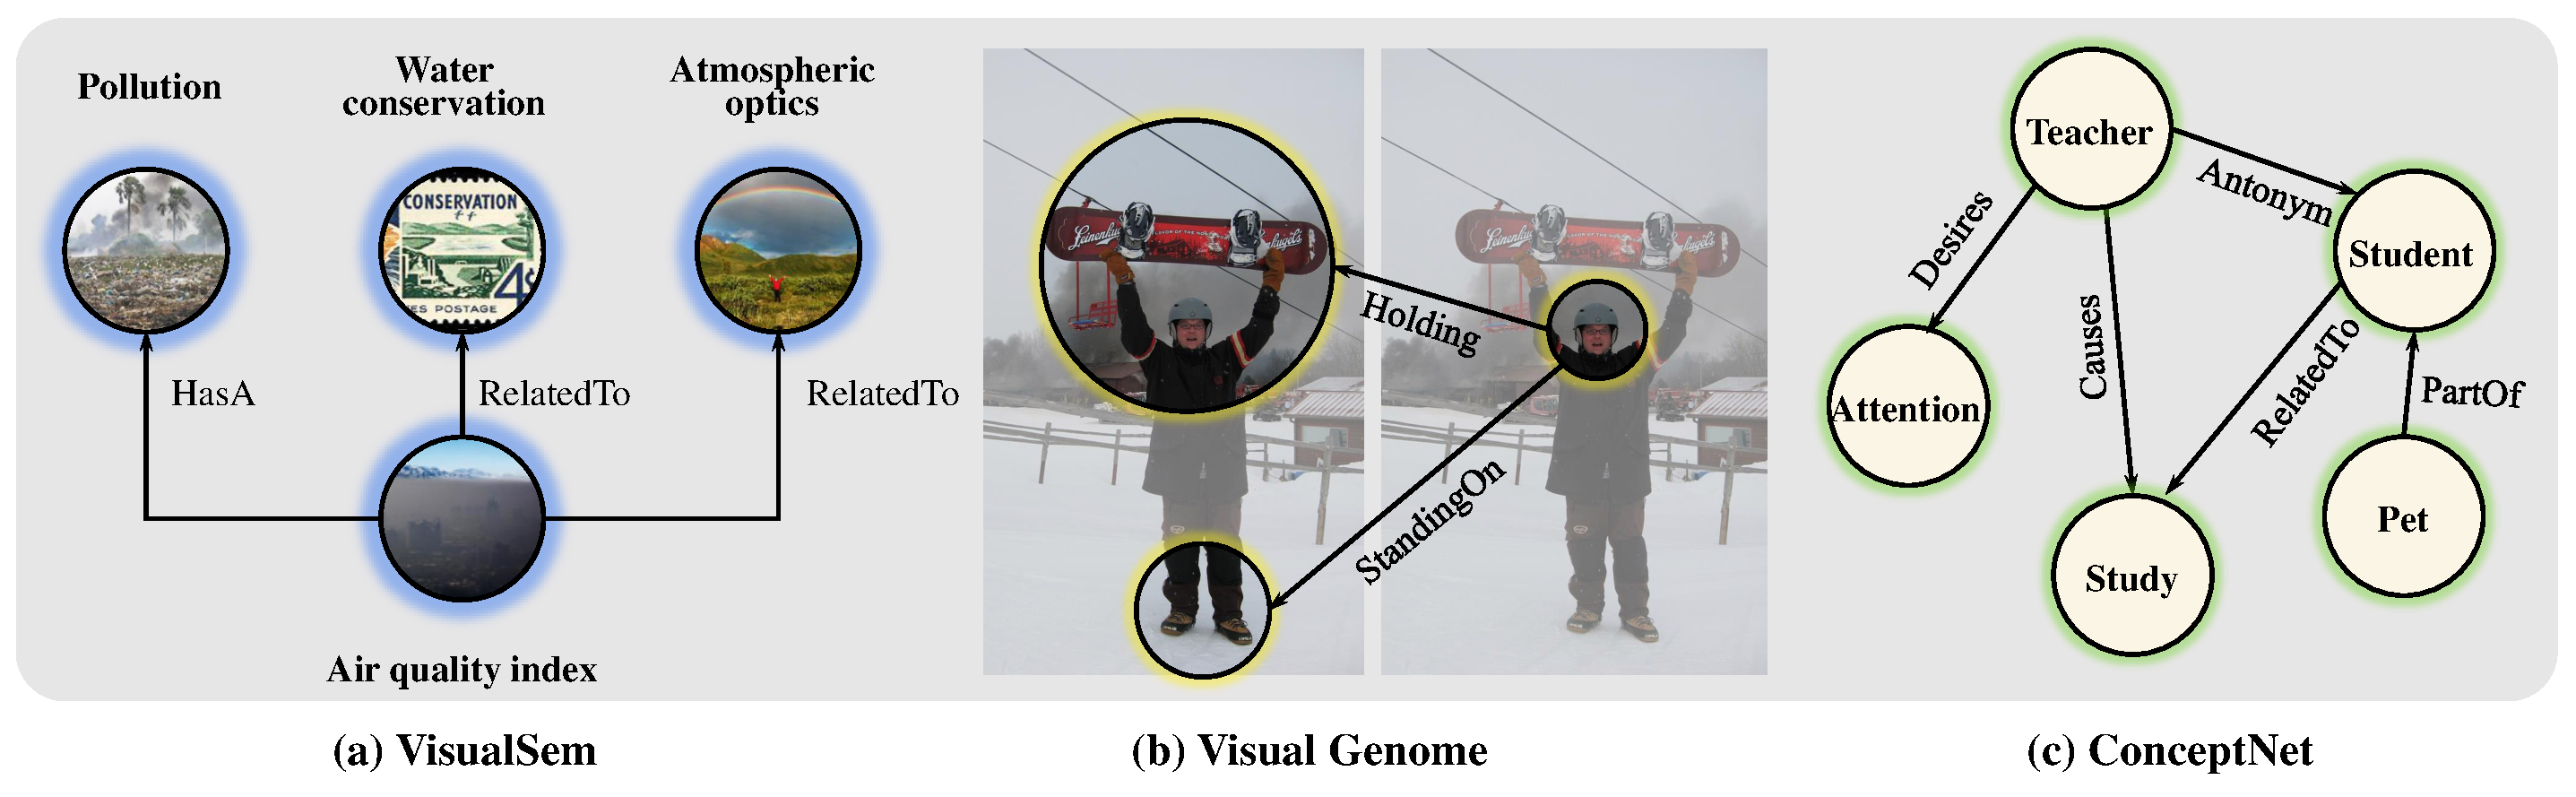
\includegraphics[width=1.0\linewidth]{3.pdf}
%   \vskip -0.1in
  \caption{Illustrations of the pre-training knowledge graph datasets, including ViusalSem~\cite{visualsem} (multi-modal graph), Visual Genome~\cite{vgdata} (scene graph), and ConceptNet~\cite{conceptnet} (language-based graph).}
  \label{fig2}
%  \vskip -0.1in  
\end{figure}

\subsection{Model Architecture}
The model architecture and the training framework are illustrated in Fig.~\ref{fig3}(A). Specifically, we first process the inputs into token sequences with modality-specific tokenizers. The BPE tokenzier~\cite{bpe} is adopted for language inputs, while image inputs are sliced into non-overlapped patches and converted into a sequence of patches following ViT~\cite{vit}. For convenient processing, we set the length of the image sequence and text sequence as $l_{\rm I}$ and $l_{\rm T}$ respectively for all inputs. To preserve the relative position information in the input, learnable positional encodings are added to the corresponding sequences before being sent to the model.

Two separate image encoder $f_{\rm I}(\cdot)$ and text encoder $f_{\rm T}(\cdot)$ are then adopted to extract features from raw inputs. For a given triplet $(h,r,t)$, the entities $h$ and $t$ are sent to the encoders with respect to their modalities (image or text). The relation $r$, which is represented by language tokens, is sent to text encoder similar to text entity. 

Compared to the model structure in CLIP, we introduce a modification to better adapt our framework. Specifically, vanilla CLIP models use a pooling function at the last layer of two encoders to compress the feature map into a global representation. Namely, for an input $u \in \mathcal{R}^{L \times d_{i}}$, where $L$ and $d_{i}$ denote the sequence length and feature dimension, the output of the encoder can be formulated as:
\begin{equation}
    x_u = f(u) \in \mathcal{R}^{L \times d_o}, \ \ \bar{x}_u = {\rm Pool}(x_u) \in \mathcal{R}^{d_o},
\end{equation}
where $f$ represents the feature extraction module, ${\rm Pool}(\cdot)$ denotes the pooling function, and $d_o$ is the output dimension. Though efficient, it also leads to inevitable information loss in the local region, especially for the image inputs. Therefore, we remove the pooling functions for image and text entities to preserve the local information, and use $x_u \in \mathcal{R}^{L \times d_o}$ as the extracted feature. The relation, on the other hand, is normally under a limited sequence length, \textit{e.g.}, one or two word tokens, where the information density is smaller than entities. Therefore, we retain the pooling function for relation input and use $\bar{x}_u \in \mathcal{R}^{d_o}$ as the extracted features.

In this way, we have extracted the features defined as $(x_h, \bar{x}_r, x_t)$, which correspond to the elements in the input triplet $(h, r, t)$. To model the joint distribution of different elements in the triplet, we consider a multi-modal encoder $\rm TransEncoder(\cdot)$ to fuse the features from different sources. Specifically, we first concatenate all the features in the triplet into a single sequence and use a head token $<\!\!{\rm head}\!\!>$ at the beginning of the sequence. To emphasize the status of the tokens in the sequence, we consider additional learnable encodings for each element $h, r, t$ in the triplet:
\begin{equation}
\label{concat}
    X(h, r, t) = [<\!\!{\rm head}\!\!>, \ x_h\!+\!{\rm PE}_h, \ \bar{x}_r\!+\!{\rm PE}_r, \ x_t\!+\!{\rm PE}_t].
\end{equation}
% We also consider the situation for incomplete triplets where certain elements are missing in the input. The concatenated sequence can be similarly derived by masking the corresponding feature. For example, the concatenated sequence for an input $(s, p, \!-\!)$ can be represented as:
% \begin{equation}
%     X(s, p, -) = [<\!\!{\rm head}\!\!>, \ x_s\!+\!{\rm PE}_s, \ \bar{x}_p\!+\!{\rm PE}_p, \ \textbf{0}].
% \end{equation}
After processing by the multi-modal encoder, the feature of the head token $<\!\!{\rm head}\!\!>$ finally serves as the representation of the whole sequence:
\begin{equation}
    Y(h, r, t) = {\rm TransEncoder}(X(h, r, t))[0, :].
\end{equation}
Also, representation for relation is extracted from the corresponding token:
\begin{equation}
\label{relout}
    R(h, r, t) = {\rm TransEncoder}(X(h, r, t))[1+{\rm len}(x_h), :].
\end{equation}

\subsection{Training Targets}
Considering the unique data structure of knowledge graphs, we mainly adopt two types of training targets in our framework, including triplet-based loss and graph-based loss as illustrated in Fig.~\ref{fig3}(B). Besides, a knowledge distillation loss is also considered due to the continuous learning strategy adopted in our framework.

\textbf{Triplet-based loss} considers a batch of triplets as the input and supervises the training of our model by estimating the joint distribution of elements in the triplets. Inspired by the mask prediction technique that models the distribution of masked tokens conditioned on the unmasked regions, we similarly mask the elements in the triplets and predict the distribution with the help of a multi-modal encoder. Specifically, for incomplete triplets where certain elements are missing in the input, the concatenated sequence can be similarly derived as in Eq.~\ref{concat} by masking the corresponding feature. For example, the concatenated sequence for an input $(h, r, \text{-})$ can be represented as:
\begin{equation}
    X(h, r, \text{-}) = [<\!\!{\rm head}\!\!>, \ x_h\!+\!{\rm PE}_h, \ \bar{x}_r\!+\!{\rm PE}_r, \ \textbf{0}].
\end{equation}

On this basis, given a set of input $D = \{(h_i, r_i, t_i)\}_{i=1}^N$, we first model the distribution when one of the entities, \textit{i.e.}, $t_i$, is masked, and derive the Entity-Entity (E2E) Loss by minimizing the negative log-likelihood:
\begin{equation}
\label{nll}
    -E_{(h,r)\sim D}{\rm log}(P(x_t|x_h,\bar{x}_r)).
\end{equation}
We practically approximate the distribution $P(x_t|x_h,\bar{x}_r)$ as the cosine similarity of $P(x_t)$ and $P(x_h,\bar{x}_r)$, and defined the loss function as:
\begin{align}
    L_{\rm E2E} = -\sum_{i=1}^N{\rm log}(\frac{{\rm exp} ({\rm cos}(Y(\text{-},\text{-},t_i), Y(h_i,r_i,\text{-}))/\tau)}{\sum_j {\rm exp} ({\rm cos}(Y(\text{-},\text{-},t_i), Y(h_j,r_j,\text{-}))/\tau)}).
\end{align}
% where
% \begin{equation}
%     s([x_{o}], [x_{s}, \bar{x}_{p}]) = {\rm cos}(Y(\!-\!,\!-\!,o), Y(s,p,\!-\!)),
% \end{equation}
% defines the similarity of masked triplets parameterized by the multi-modal encoder defined in Eq.(6).

We also model the distribution when the relation in the triplet is masked, and similarly derive the Entity-Relation (E2R) Loss:
\begin{equation}
    -E_{(h,t)\sim D}{\rm log}(P(\bar{x}_r|x_h,x_t)).
\end{equation}
Different from E2E loss, the relations in the triplets are defined in a limited set of relation groups. Therefore, we instead extract the representation of relation through an auxiliary two-layer MLP network, and model the objective as a classification problem from a predefined set of relation labels $\mathcal{R}$. In this way, the loss function can be defined as:
\begin{equation}
    L_{\rm E2R} = -\sum_{i=1}^N \sum_{r\in \mathcal{R}} \mathbf{1}_{(r=r_i)} {\rm log}(y(\bar{x}_{r_i})), \ \ {\rm where} \ \  y(\bar{x}_{r_i}) = {\rm MLP}(R(h_i,\text{-},t_i)),
\end{equation}
is extracted from an MLP model followed by the output of multi-modal encoder defined in Eq.~(\ref{relout}).

\textbf{Graph-based loss.} We also take advantage of the graph structure in knowledge graph datasets, and adopt a graph neural network to extract deeper structural information among entities. We propagate information through connected edges in the graph, and update entity representations with aggregated feature. Specifically, for a graph neural network with $L$ layers, the update function for the $l_{\rm th}$ layer can be formulated as:
\begin{align}
    G^{(l)}(t) = E_{\{h_i,r_i,t\} \in \mathcal{T_R}} \ & g^{(l-1)}(R(h_i,\text{-},t))G^{(l-1)}(h_i), \ \ G^{0}(t) = Y(\text{-},\text{-},t),\\
     {\rm where} &\ \ g^{(l)}(R(h_i,\text{-},t))=W^{(l)}R(h_i,\text{-},t),
\end{align}
calculates the aggregation weights by relation representation $R(h_i,\text{-},t)$ with a learnable matrix $W^{(l)}$.

Finally, we define the Graph-Entity(G2E) Loss by computing the cosine similarity of entity features before and after the propagation procedure in the graph:
\begin{align}
    L_{\rm G2E} = -\frac{1}{\mathcal{N}_{\xi}} \sum_{t_i \in \xi} {\rm log}(\frac{{\rm exp} ({\rm cos}(Y(\text{-},\text{-},t_i),G^{(L)}(t_i))/\tau)}{\sum_{t_j} {\rm exp} ({\rm cos}(Y(\text{-},\text{-},t_i),G^{(L)}(t_j))/\tau)}).
\end{align}

\textbf{Continuous Learning.} Large-scale pre-training usually requires massive computation resources which makes it highly inefficient when training from scratch. Therefore, to inject the semantic information in an efficient manner, we consider training our model based on the pre-trained weights from the original CLIP. This powerful initialization promotes the convergence of our model and greatly enhances the training efficiency. However, naively extending the training process with new data leads to severe forgetting problem that hampers the performance of the original models. 

To address this limitation, we adopt simple solutions to maintain CLIP performances while improving its ability to extract semantic features from knowledge graphs. (1) Besides the knowledge graph datasets, we also train our model on several widely adopted image-text datasets that share a similar data distribution with the training data in CLIP. To better fit our pre-training framework, we convert the original image-text pair into the form of triplets, with specifically designed relations 'image of' and 'caption of'. (2) We also use the original CLIP model as the teacher, and use an auxiliary loss $L_{\rm KD}$ to measure the KL distance between the output of CLIP and our model.

Overall, the final pre-training objective of Knowledge-CLIP is formulated as:
\begin{equation}
    L = L_{\rm E2E} + L_{\rm E2R} + L_{\rm G2E} + L_{\rm KD}.
\end{equation}

% \textbf{Learning Rate Adjustment.} As the added multi-modal encoder is trained from random initialization, we also decrease the learning rate for the pre-trained weights from CLIP to achieve a more balanced step in the optimization.
